%**
%*  @file  cloudnv.tex
%*  @brief  DIET Programmer' guide, Diet Cloud submission
%*  @author  Yulin Zhang (huaxi.zhang@ens-lyon.fr) 
%*  @section Licence 
%*    |LICENSE|
The chapter presents the entire design decisions of Diet on cloud area.

\section{Design diagrams}
\subsection{SedCloud types}
 A SedCloud can have four different ways to instantiate itself and Vms. Figure illustrates an activity diagram of the three possibilities.
\begin{enumerate}
\item SedCloud with temporary VMs accoridng to solve requests
\item SedCloud with persistent VMs according to the first solve request
\item SedCloud with persistent Vms initiated at the same time
\item SedCloud without any VM
\end{enumerate}

\begin{figure}[!htb]
  \centering
  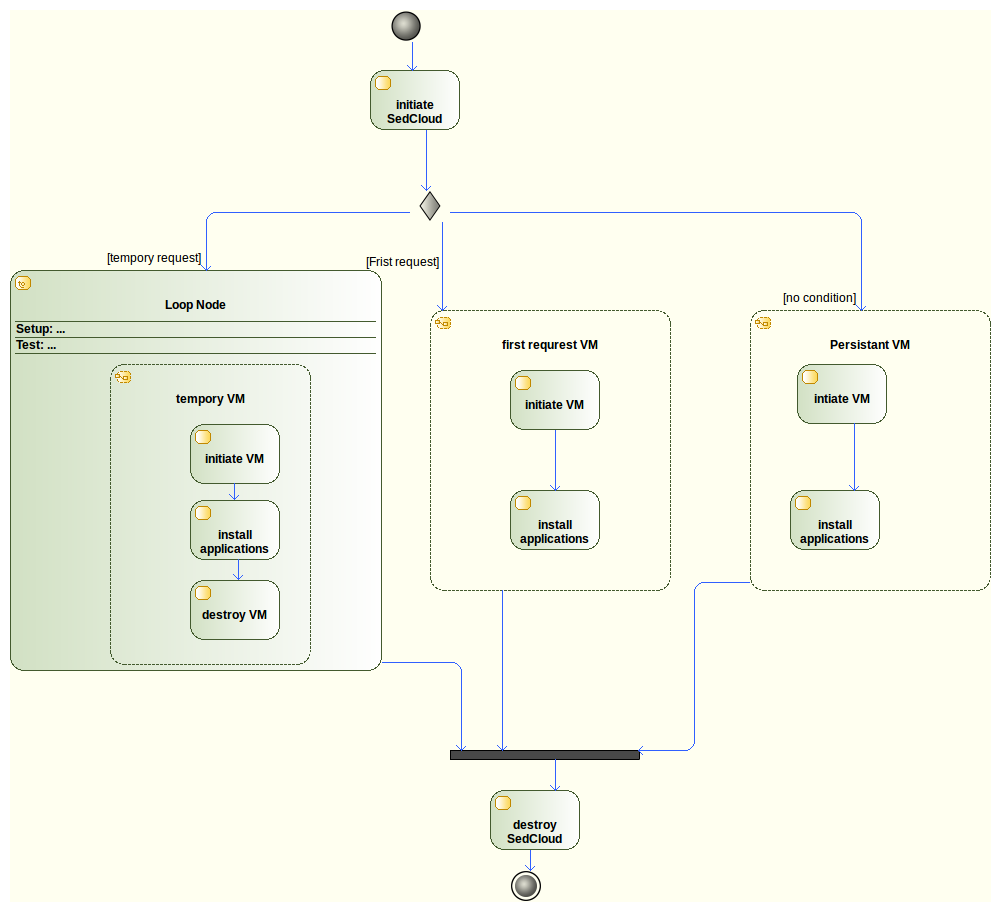
\includegraphics[width=0.8\textwidth]{fig/ActivityDiagramSedCloud.png}
  \caption{Four types of SedCloud} \label{fig:SedCloudTypes}
\end{figure}

\subsection{SedCloud communication}
The simple diagram of SedCloud communication is presented in Figure~\ref{fig:SedCloudcommunication}. 
\begin{itemize}
\item DeltaCloud is just used to instantiate or destroy a VM in cloud.
\item The commnucation for applications at this moment is directly between SedCloud and Vms. 
\end{itemize}

\begin{figure}[!htb]
  \centering
  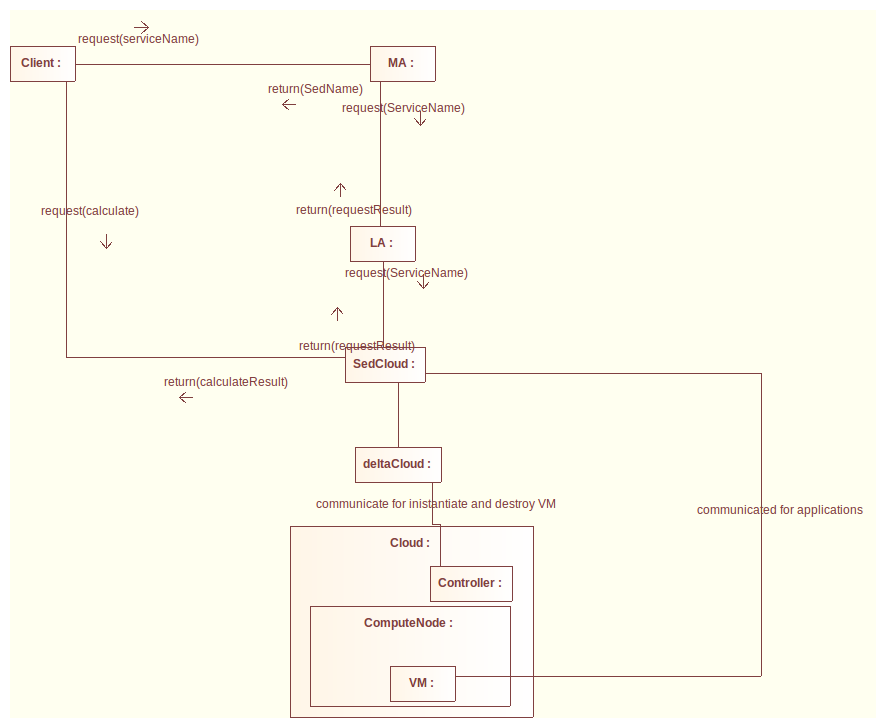
\includegraphics[width=0.8\textwidth]{fig/communicationDiagramSedCloud.png}
  \caption{Communication between Client, MA, LA and SedCloud} \label{fig:SedCloudcommunication}
\end{figure}